\chapter{PENDAHULUAN}

\section{Latar Belakang}

Indonesia merupakan negara maritim dengan luas laut dan perairan 62\% \parencite{inproc:wuryadani}. Potensi ini harus didukung berdasarkan prinsip \textit{Blue Economy}. \textit{Blue Economy} sendiri merupakan komponen penting dalam pengembangan keberlanjutan yang berfokus pada ekonomi maritim yang meliputi berbagai sektor seperti perikanan, akuakultur, dan transportasi maritim. Konsep \textit{Blue Economy} berkaitan erat dengan \textit{Sustainable Development Goal} ke 14 yang membahas mengenai pelestarian dan penggunaan lautan, laut, dan sumber daya laut secara berkelanjutan \parencite{misc:lse}. Menurut \textcite{misc:dephub}, transportasi laut memegang peran strategis untuk mendorong pertumbuhan ekonomi di Indonesia. Salah satu bentuk untuk mendukung rencana jangka panjang ini adalah melalui upaya menuntaskan permasalahan fundamental dari industri tersebut. Pada industri maritim, salah satu biaya dengan rasio komposisi terbesar terletak pada biaya bahan bakar operasional. Tingginya biaya bahan bakar ini dapat memperlambat kemajuan industri maritim dikarenakan akan mengurangi pendapatan perusahaan, terlebih jika ternyata tingginya biaya bahan bakar ini disebabkan oleh hal lain diluar operasional. Sehingga, memastikan bahwa penggunaan bakar lebih efisien dirasa perlu.

Efisiensi sendiri terbagi menjadi dua, yakni Efisiensi Teknologi dan Efisiensi Manajemen. Efisiensi Teknologi merujuk pada keterbaruan teknologi mesin yang mampu menghemat penggunaan bahan bakar dari waktu ke waktu. Sedangkan pada Efisiensi Manajemen memastikan bahwa bahan bakar sepenuhnya digunakan untuk mendukung operasi. Fokusan pada penelitian ini adalah Efisiensi Manajemen. Untuk itu, diperlukan sebuah teknologi untuk melakukan validasi data penggunaan bahan bakar yang dilaporkan dengan nilai aktual yang dihabiskan.

Teknologi transformatif tersebut bernama IoT atau \textit{Internet of Things} yang berpotensi merevolusi berbagai industri melalui kontrol dan pemantauan ekstensif secara jarak jauh \parencite{article:hercog}. Kemampuan teknologi IoT dalam memberikan data secara jarak jauh membuka jalan bagi pelaku industri untuk merealisasi efisiensi bahan bakar khususnya pada transportasi laut. Hal ini senada dengan penelitian yang dilakukan \textcite{article:suciu}, yang menyatakan IoT memungkinkan integrasi mesin, sistem, dan proses untuk meningkatkan efisiensi operasional dan \textit{predictive maintenance}.

Langkah untuk melakukan efisiensi dengan kontrol melalui teknologi IoT juga dinilai tepat mengingat minyak fosil akan habis di tahun 2070 \parencite{misc:bp} sehingga pelaku industri tidak hanya menghemat biaya operasional, tetapi secara tidak langsung juga menjaga lingkungan secara berkelanjutan. Dengan demikian, operasi akan dipastikan berjalan secara optimal dengan memanfaatkan bahan bakar secara maksimal. Sebaliknya, salah satu dampak yang ditimbulkan dari belum diterapkannya teknologi ini adalah kurangnya kontrol yang mengakibatkan celah pada pelanggaran hukum. Pada tahun 2020 terdapat kasus penggelapan bahan bakar yang mencapai 2.5 ton liter \parencite{misc:aditya}, sehingga menimbulkan kerugian negara mencapai 710 juta rupiah. Hal ini dapat diatasi menggunakan sistem monitoring berbasis IoT yang memungkinkan pemantauan secara jarak jauh. Sistem monitoring berbasis IoT yang dimaksud adalah suatu sistem yang menggunakan \textit{Internet of Things} untuk memantau dan menyimpan data dari berbagai sensor. Dalam penelitian ini maka akan dikembangkan Sistem Monitoring berbasis IoT yang akan bekerja sama dengan salah satu perusahaan swasta yang bergerak di bidang transportasi laut sebagai mitra, yaitu PT Bisma Jaya.

PT Bisma Jaya merupakan perusahaan jasa maritim yang menyediakan berbagai jenis kapal untuk kebutuhan transportasi laut. Berdasarkan informasi yang diperoleh dari Direktur Operasional perusahaan, saat ini digunakan laporan harian dan bulanan sebagai acuan dalam mengestimasi jumlah bahan bakar yang diperlukan di bulan berikutnya. Permasalahan yang umum terjadi adalah waktu sampai yang lebih lama dari estimasi dan sulitnya mengontrol konsumsi bahan. Sistem Monitoring berbasis IoT dinilai cocok untuk menuntaskan permasalahan tersebut, dimana sistem memungkinkan pemantauan data kecepatan mesin dan bahan bakar secara jarak jauh agar sesuai dengan ketentuan yang berlaku, memastikan penggunaan bahan bakar termanfaatkan dengan maksimal.

Untuk merealisasi penelitian ini dibutuhkan lintas disiplin ilmu, yakni elektronika dan komputer. Oleh karena itu, dibutuhkan suatu metode pengembangan sistem yang lebih menekankan kolaborasi serta komunikasi yang baik. Terdapat metode \textit{Waterfall}, yang merupakan proses desain sekuensial yang digunakan dalam proyek pengembangan perangkat lunak. Ini mengikuti perkembangan linier melalui fase yang berbeda, termasuk pengumpulan dan analisis kebutuhan, desain, pengkodean, pengujian, dan pemeliharaan \parencite{article:abbas}. Metode ini, mengasumsikan kebutuhan telah final di awal proyek, serta tiap fase harus diselesaikan terlebih dahlu sebelum lanjut ke fase berikutnya. Oleh karenanya, metode ini tidak cocok untuk diterapkan pada sistem yang memiliki kebutuhan yang dinamis. Sehingga, penggunaan metode \textit{Waterfall} dirasa kurang cocok dalam pengembangan Sistem Monitoring berbasis IoT dikarenakan sulitnya untuk mengatur perubahan dan beradaptasi pada kebutuhan yang berkembang.

\textit{Agile} merupakan pendekatan yang secara efektif dapat beradaptasi dengan kebutuhan yang berubah-ubah, yang mana ini sulit untuk diatur pada model \textit{Waterfall}. Salah satu metode yang populer adalah Scrum. Scrum merupakan metodologi yang berfokus pada pengembangan berulang dan bertahap, fleksibilitas, dan perbaikan terus menerus. Metodologi ini sangat cocok untuk pengembangan proyek skala masif dengan personel pengembang yang banyak.

Lalu terdapat metode \textit{Extreme Programming} (XP), sebuah metode \textit{agile} yang menekankan pada kolaborasi, adaptasi, dan pengembangan iteratif \parencite{article:matharu}. \textit{Extreme Programming} metode yang ideal untuk digunakan tim skala kecil menengah dalam pengembangkan perangkat lunak dengan cepat serta fleksibel dalam menghadapi perubahan. Salah satu prinsip dari metode ini adalah keterlibatan pelanggan \parencite{article:matharu}. Hal ini memastikan perangkat lunak memenuhi kebutuhan pelanggan dan mengurangi risiko pengembangan fitur yang tidak diperlukan.

Berdasarkan pertimbangan pilihan metode yang sudah dilakukan, metode yang paling cocok untuk diterapkan pada studi kasus penelitian ini adalah metode \textit{Extreme Programming} (XP) karena dari perusahaan membutuhkan sistem yang dapat dengan cepat diimplementasikan tanpa harus melalui proses dokumentasi yang banyak. Metode ini cocok untuk pengembangan sistem dengan tim yang sedikit dan dalam kurun waktu yang relatif singkat, serta bersifat fleksibel terhadap perubahan dikarenakan adanya kemungkinan perubahan kebutuhan terkait fitur-fitur yang ada pada sistem.

Diharapkan dengan adanya penelitian ini, Sistem Monitoring pada mesin diesel yang dikembangkan dapat membantu PT Bisma Jaya khususnya Direktur Operasional dalam melakukan pemantauan penggunaan bahan bakar serta menjaga efektivitas armada kapal yang sedang beroperasi yang mulanya melalui laporan harian/bulanan yang dibuat secara manual menjadi sistem yang dapat menyajikan data historis dan dapat diakses kapan saja.



\section{Rumusan Masalah}

Berdasarkan latar belakang dari penelitian, didapatkan rumusan masalah sebagai berikut.

\begin{enumerate}
    \item Bagaimana sistem monitoring dirancang menggunakan metode \textit{Extreme Programming}?
    \item Bagaimana sistem monitoring dikembangkan menggunakan metode \textit{Extreme Programming}?
\end{enumerate}

\section{Tujuan}

Tujuan dari penelitian ini adalah sebagai berikut.

\begin{enumerate}
    \item Untuk merancang sistem monitoring menggunakan metode \textit{Extreme Programming}.
    \item Untuk mengembangkan sistem monitoring menggunakan metode \textit{Extreme Programming}.
\end{enumerate}

\section{Manfaat}

Manfaat yang didapatkan pada penelitian ini adalah sebagai berikut.

\begin{enumerate}
    \item Membantu perusahaan dalam melakukan pengawasan dan kontrol konsumsi bahan bakar armada kapal selama operasi.
    \item Membantu perusahaan dalam memastikan efektivitas operasi
\end{enumerate}


\section{Batasan Penelitian}

Batasan penelitian ini adalah sebagai berikut.

\begin{enumerate}
    \item Fokus utama pada penelitian ini adalah pengembangan Sistem Monitoring berbasis web
    \item Pada penelitian ini diterapkan 3 layer arsitektur IoT teratas: \textit{App Layer}, \textit{Data Processing Layer}, dan \textit{Network Layer}
    \item Sistem Monitoring berbasis IoT dikembangkan menggunakan framework
    NextJS, Django, dan MySQL sebagai \textit{Database Management Systems (DBMS)}
\end{enumerate}
\section{Kerangka Pemikiran Penelitian}

Berikut kerangka pikiran pada penelitian ini.

\begin{figure}[ht]
    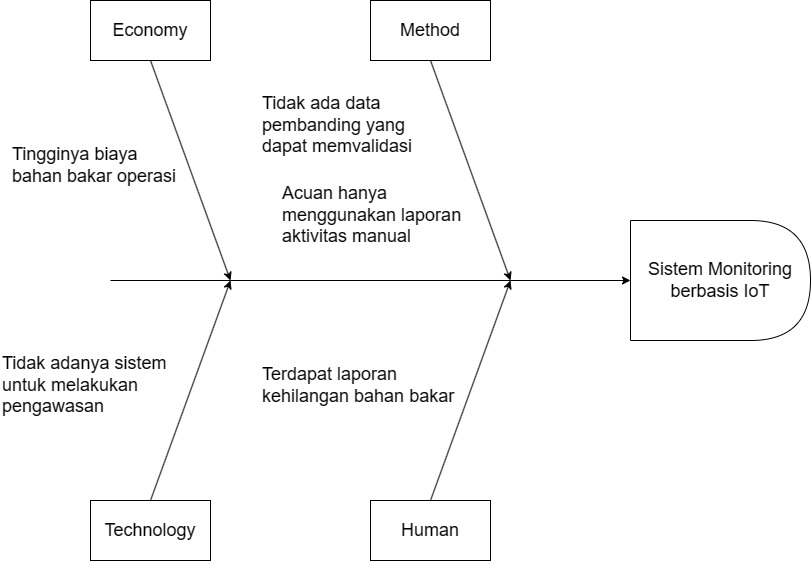
\includegraphics[width=1\linewidth, center]{images/pendahuluan/fig-framework-penelitian.jpg}
    \caption{Kerangka Penelitian}
    \label{fig:thinking-framework}
\end{figure}

\newpage

Gambar 1.1  merupakan kerangka pemikiran penelitian yang bertujuan untuk memberikan gambaran mengenai urgensi implementasi Sistem Monitoring berbasis \textit{Internet of Things (IoT)} di PT Bisma Jaya. Perusahaan ini dihadapkan pada masalah utama berupa tingginya pengeluaran untuk bahan bakar selama operasionalnya, yang dipengaruhi oleh sejumlah permasalahan dalam aspek-aspek ekonomi, metode, teknologi, dan manusia.

Kategori ekonomi, laporan harian secara rutin dibuat setiap malamnya oleh tim operasional kapal. Selama operasi, mereka menjaga catatan aktivitas dalam sebuah jurnal yang mencatat waktu perjalanan dan berhenti kapal. Namun, terdapat kekurangan dalam pencatatan yaitu tidak adanya pencatatan jumlah jam operasi pada tiap kategori operasi tertentu. Akibatnya, ketika mereka membuat laporan, nilai \textit{running hour} untuk tiap kategori operasi hanya dapat diestimasikan saja, yang bisa berpotensi mengakibatkan perhitungan konsumsi bahan bakar lebih tinggi dari seharusnya. Informasi lebih lanjut mengenai kategori operasi dapat dilihat pada Bab \ref{ch:2} bagian \ref{sec:fcrv}.

Kategori metode, perusahaan selama ini mengandalkan laporan bulanan yang dibuat tim operasional kapal. Hanya saja, tidak ada data faktual yang dapat dijadikan pembanding terhadap laporan yang dibuat. Selain itu, laporan tersebut baru diterima setiap akhir bulan, sehingga perusahaan tidak memiliki data apapun hingga mendapat temuan dari pihak pengguna.

Kategori teknologi, tidak adanya suatu sistem monitoring yang dipasang pada armada juga menjadi salah satu masalah utama perusahaan. Selama ini, perusahaan hanya mengandalkan data dari AVTS untuk mengetahui data \textit{running hour}, kecepatan (knot), dan posisi kapal. Tetapi, alat ini tidak dapat memberikan informasi detail terkait kecepatan mesin dan konsumsi bahan bakar.

Kategori manusia, pengguna jasa perusahaan telah mengalami situasi di mana mereka melaporkan adanya kejadian kehilangan bahan bakar. Sebelum armada kapal mengisi ulang bahan bakarnya, operator \textit{fuel management} pengguna jasa akan melakukan pengukuran yang dikenal dengan istilah "sounding." Hasil dari pengukuran ini akan dibandingkan dengan laporan harian yang disusun oleh tim operasional kapal. Apabila ditemukan selisih sebesar lebih dari 100 liter, operator \textit{fuel management} akan melaporkan indikasi kehilangan yang dapat mengakibatkan dikenakan denda.

Secara garis besar, didapatkan inti permasalahan yang terjadi di PT Bisma Jaya adalah belum adanya langkah kontrol pada bahan bakar pada kapal yang dimiliki, sehingga pada penelitian ini akan dikembangkan Sistem Monitoring mesin diesel yang akan membantu perusahaan dalam melakukan pemantauan jumlah bahan bakar selama operasi.